\section{Objective}
The objective of this experiment is to investigate the behavior of second-order systems, namely, the RLC circuit. During the lab, various RLC circuit configurations are built and theoretical results are compared with experimental results with the aid of MATLAB.

\section{Introduction}
Second order systems are very common, named due to the highest order of the differential equation describing the system. For an RLC circuit, we tend to use a second-order ordinary differential equation to describe the system, which is given by

\begin{equation}
    a_2 \frac{d^2 y(t)}{dt^2} + a_1 \frac{dy(t)}{dt} + a_0 y(t) = x(t)
\end{equation}
Where we define $y(t)$ as the output of the system, $x(t)$ as the input of the system, and $a_2$, $a_1$, and $a_0$ as system parameters.

However, in the context of the response of second-order systems we tend to use a more general form of this equation, given by

\begin{equation}
    \frac{d^2 y(t)}{dt^2} + 2 \zeta \omega_n \frac{dy(t)}{dt} + \omega_n^2 y(t) = K \omega_n^2 x(t)
\end{equation}

Where we now define the system parameters as:

\begin{itemize}
    \item $\zeta$ - damping ratio
    \item $\omega_n$ - natural frequency
    \item $K$ - gain of the system
\end{itemize}

For second order differential equations, we know that $y_t = y_p + y_h$ where $y_p$ is the particular solution and $y_h$ is the homogeneous solution.

To solve for the homogenous solution, we set the input to zero and solve the differential equation. The general solution for the homogenous solution is given by
\begin{equation}
    y_h(t) = C_1 e^{\lambda_1 t} + C_2 e^{\lambda_2 t}
\end{equation}
Where $C_1$ and $C_2$ are constants defined by initial conditions and $\lambda_1$ and $\lambda_2$ are the roots of the characteristic equation that are determined by the resistor, capacitor, and inductor values.

We know that depending on $\zeta$ and the undamped natural frequency $\omega_n$ we can classify the transient response of the system into three categories:
\begin{itemize}
    \item Overdamped - $\zeta > 1$
    \item Critically damped - $\zeta = 1$
    \item Underdamped - $\zeta < 1$
\end{itemize}

Each of these categories has a different equation, which are given below:


\begin{enumerate}
    \item {\bf Overdamped}

          In the overdamped case, the response is the sum of two decaying exponentials, defined as
          \begin{equation}
              y(t) = C_1 \exp{
                  \left(\left(-\zeta + \sqrt{\zeta^2 - 1}\right) w_nt\right)
              } + C_2 \exp{
                  \left(\left(-\zeta - \sqrt{\zeta^2 - 1}\right) w_nt\right)
              }
          \end{equation}
    \item {\bf Critically damped}

          In the case of critical damping, the system reaches steady state in the shortest amount of time, the equation given by the state below.
          \begin{equation}
              y(t) = C_1 e^{\lambda_1 t} + C_2 t e^{\lambda_2 t}
          \end{equation}
          \newpage
    \item {\bf Underdamped}
          \begin{figure}[H]
              \centering
              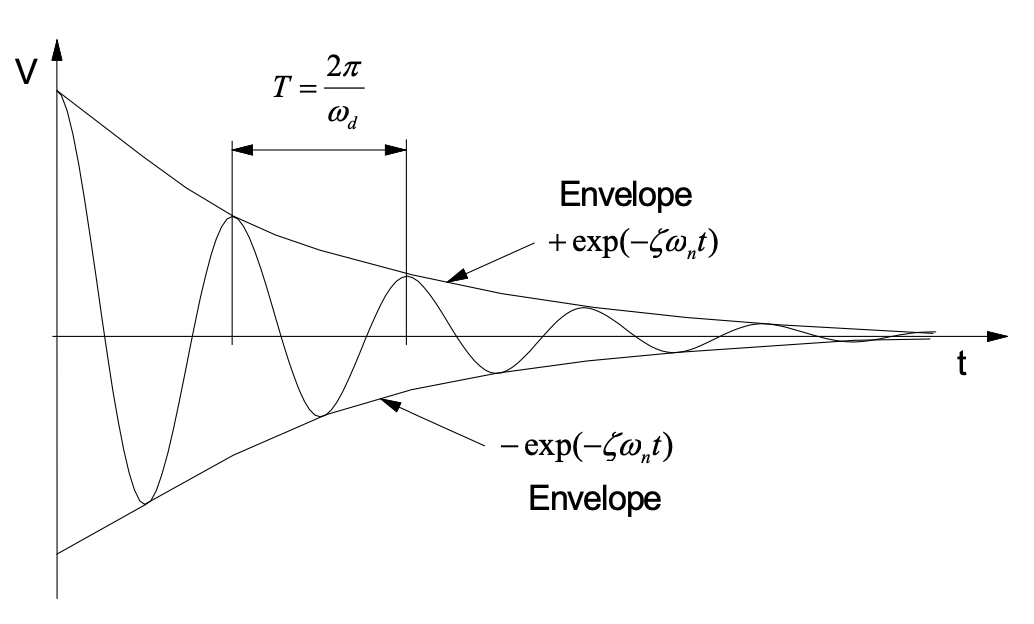
\includegraphics[width=0.5\textwidth]{images/underdamped_intro_behaviour.png}
              \caption{Underdamped Response}
              \label{fig:underdamped_envelope}
          \end{figure}

          In the underdamped case, we can observe ringing in the response. This is due to the fact that the system is oscillating around the steady state value.

          For the underdamped case, let's consider $w_d$ as the damped natural frequency, given by $w_d = w_n \sqrt{(1-\zeta^2)}$. We can then write the equation as
          \begin{equation}
              y(t) = e^{-\zeta \omega_n t} \left(C_1\cos\left(w_dt\right) + C_2\sin\left(w_dt\right) \right)
          \end{equation}
\end{enumerate}
\begin{figure}[H]
    \centering
    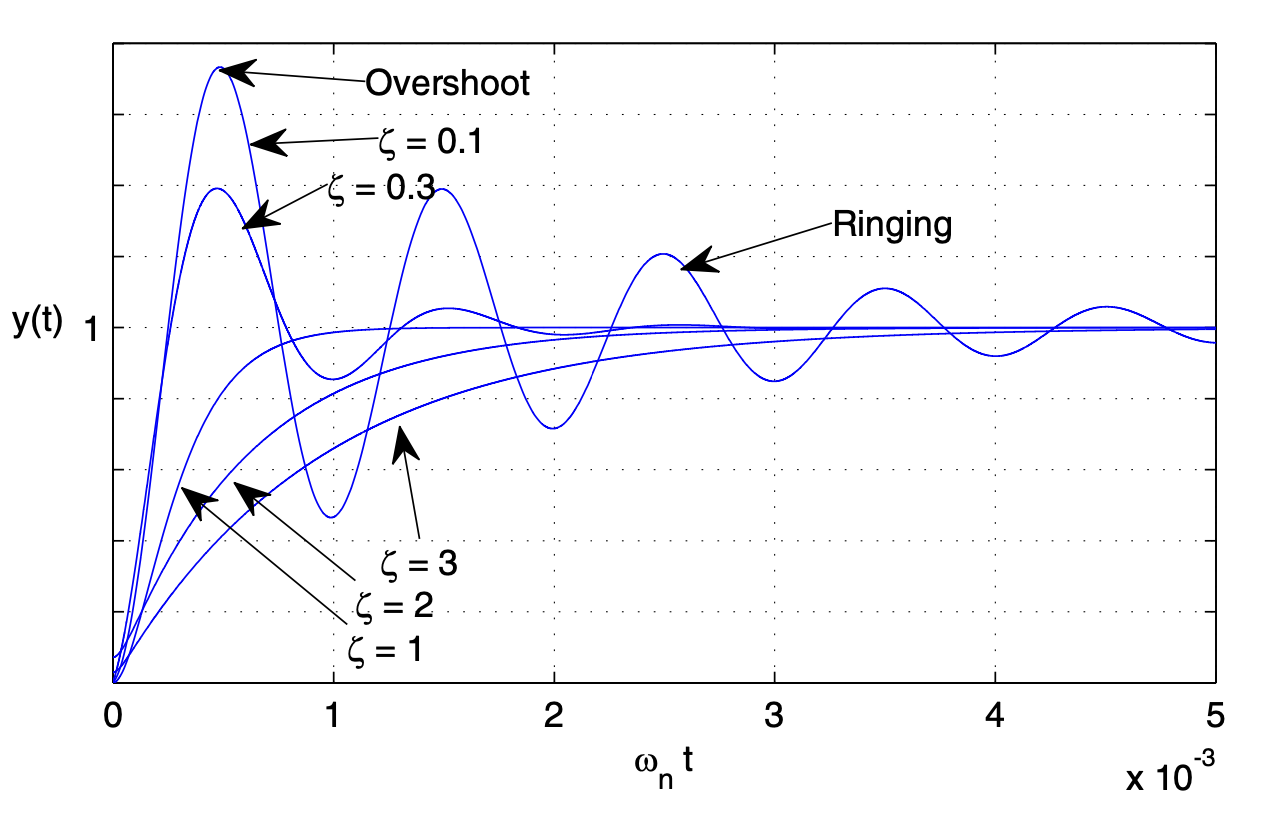
\includegraphics[width=0.45\textwidth]{images/general_intro_behaviour.png}
    \caption{General Transient Response Diagram}
    \label{fig:general_transient_response}
\end{figure}
Below is a figure that shows the cases of the transient response of a second order system according to the damping ratio $\zeta$ when provided with a step input.

Considering a forced solution is out of the scope of this lab, but in general, the output will usually be a weighted sum of the input signal $x(t)$ and its first and second derivatives.